
%(BEGIN_QUESTION)
% Copyright 2005, Tony R. Kuphaldt, released under the Creative Commons Attribution License (v 1.0)
% This means you may do almost anything with this work of mine, so long as you give me proper credit

An interesting technology dating back at least as far as the 1940's, but which is still of interest today is {\it power line carrier}: the ability to communicate information as well as electrical power over power line conductors.  Hard-wired electronic data communication consists of high-frequency, low voltage AC signals, while electrical power is low-frequency, high-voltage AC.  For rather obvious reasons, it is important to be able to separate these two types of AC voltage quantities from entering the wrong equipment (especially the high-voltage AC power from reaching sensitive electronic communications circuitry).

Here is a simplified diagram of a power-line carrier system:

$$\includegraphics[width=15.5cm]{i01214x01.eps}$$

The communications transmitter is shown in simplified form as an AC voltage source, while the receiver is shown as a resistor.  Though each of these components is much more complex than what is suggested by these symbols, the purpose here is to show the transmitter as a {\it source} of high-frequency AC, and the receiver as a {\it load} of high-frequency AC.

Trace the complete circuit for the high-frequency AC signal generated by the ``Transmitter'' in the diagram.  How many power line conductors are being used in this communications circuit?  Explain how the combination of ``line trap'' $LC$ networks and ``coupling'' capacitors ensure the communications equipment never becomes exposed to high-voltage electrical power carried by the power lines, and vice-versa.

\underbar{file i01214}
%(END_QUESTION)





%(BEGIN_ANSWER)

$$\includegraphics[width=15.5cm]{i01214x02.eps}$$

\vskip 10pt

Follow-up question \#1: trace the path of line-frequency (50 Hz or 60 Hz) load current in this system, identifying which component of the line trap filters ($L$ or $C$) is more important to the passage of power to the load.  Remember that the line trap filters are tuned to resonate at the frequency of the communication signal (50-150 kHz is typical).

\vskip 10pt

Follow-up question \#2: coupling capacitor units used in power line carrier systems are special-purpose, high-voltage devices.  One of the features of a standard coupling capacitor unit is a {\it spark gap} intended to ``clamp'' overvoltages arising from lightning strikes and other transient events on the power line:

$$\includegraphics[width=15.5cm]{i01214x03.eps}$$

Explain how such a spark gap is supposed to work, and why it functions as an over-voltage protection device.

%(END_ANSWER)





%(BEGIN_NOTES)

Although power line carrier technology is not used as much for communication in high-voltage distribution systems as it used to be -- now that microwave, fiber optic, and satellite communications technology has superseded this older technique -- it is still used in lower voltage power systems including residential (home) wiring.  Ask your students if they have heard of any consumer technology capable of broadcasting any kind of data or information along receptacle wiring.  ``X10'' is a mature technology for doing this, and at this time (2004) there are devices available on the market allowing one to plug telephones into power receptacles to link phones in different rooms together without having to add special telephone cabling.

Even if your students have not yet learned about three-phase power systems or transformers, they should still be able to discern the circuit path of the communications signal, based on what they know of capacitors and inductors, and how they respond to signals of arbitrarily high frequency.

Information on the coupling capacitor units was obtained from page 452 of the {\it Industrial Electronics Reference Book}, published by John Wiley \& Sons in 1948 (fourth printing, June 1953).  Although power line carrier technology is not as widely used now as it was back then, I believe it holds great educational value to students just learning about filter circuits and the idea of mixing signals of differing frequency in the same circuit.

%INDEX% Electronics review: powerline carrier

%(END_NOTES)


